\documentclass[11pt]{article}
\usepackage{local}
\title{\bf The IceCube Experiment}
\author{Yutong Du}
\date{\vspace{2px} \hrule \vspace{-0.2in}}
\fontfamily{pbk} 
\usepackage{cleveref}
\usepackage{times}
\usepackage{titling}
\setlength{\droptitle}{-0.75in}
\linespread{1.1}
\usepackage[style=numeric,sorting=none,maxnames=3]{biblatex}
\addbibresource{references.bib}
\begin{document}
\maketitle

\begin{abstract}
    \noindent This research paper is focused on the IceCube experiment, a particle detector located 
    at the South Pole. In this paper, I will discuss the motivations behind the 
    construction of such a detector, the detector instrumentation and specifics about 
    the detectors themselves, then discuss future plans the IceCube collaboration 
    has lined out. I'm confined to only three pages of material, so I will only 
    be able to a very general overview into this topic; references are at the end 
    of the document for further reading.
\end{abstract}
    \section{Introduction}
    IceCube is a Cherenkov neutrino detector located at the south pole that completed 
    construction in 2009. At over 2km in depth, it currently holds the title of the 
    largest neutrino observatory in the world. Currently, research at IceCube is focused
    on studying cosmic rays and astrophysical neutrinos -- that is, neutrinos that come from deep
    space rather than from the sun.

    One of the primary motivations for the IceCube detector was the fact that in order to 
    truly study high energy cosmic neutrinos, we would first need to build a kilometer-scale 
    detector which could measure them. Traditionally, this would require a large
    amount of water (or other medium for detection), and consequently an enormous vessel
    to contain it. However, one of the main advantages of IceCube is that there is no 
    need to build such a vessel. Instead, the ice itself acts as the medium for 
    detection, and as a result we are able to build a significantly large detector at a 
    relatively low cost, especially when compared to the traditional methods which require the vessel. In addition to this, building 
    a detector at the south pole makes it a relatively isolated environment, which is 
    great for detection purposes, since this naturally reduces the noise level and allows
    for more precise measurements.

    \section{Structure}
    Before building IceCube, we needed to first demonstrate that using antarctic
    ice as a detector was actually viable -- this was the goal of the Antarctic Muon And
    Neutrino Detector Array, or AMANDA for short. AMANDA was a relatively small scale
    detector that used photomultiplier tubes (PMTs) attached to strings that penetrated deep
    into the ice, which detected the Cherenkov light that neutrino interactions with
    the ice would produce. From 2000 to 2009, AMANDA provided convincing evidence that 
    the antarctic ice was was certainly a viable medium to make neutrino detections with 
    -- as a result of their conclusions, the experiment was then expanded dramatically 
    into the kilometer-scale detector known today as IceCube. 

    While IceCube is generally used to refer to the experiment as a whole, it's important 
    to note that IceCube is in fact only one of three main components. The other two are 
    IceTop, which refers to the surface array, and DeepCore, a region within the detector
    with a higher density of PMTs. Macroscopically, the arrangement of the PMTs has not 
    changed, only now there are many more of them and are also spread out over a 
    very large area. 


    \subsection{IceTop}
    IceTop is one of the three data-taking instruments at the IceCube detector. Completed 
    in 2010, it focuses primarily on the detection of air showers: atmospheric particles that are
    created as a result of interactions between astrophysical cosmic rays and the Earth's
    atmosphere. It also serves as a calibration detector for IceCube. 
 \begin{figure}
        \centering
        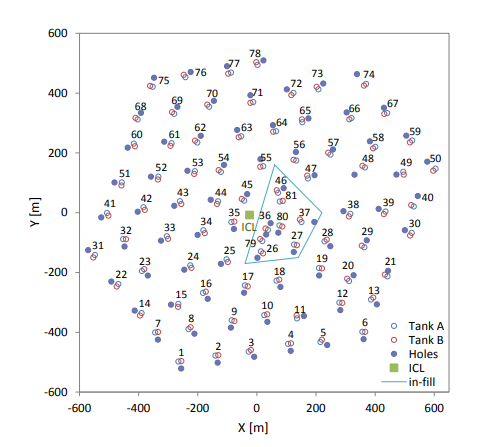
\includegraphics[scale=0.46]{icecube-arr.png}
        \caption{Schematic of IceCube Arrangement. Notice that the locations of the tanks and 
        the holes (solid dots) which contain IceCube's detectors all follow the same 
        grid-like pattern.}
        \label{icecube-arr}
    \end{figure}
    IceTop consists of an array of 81 stations located in the same grid-like arrangement
    that IceCube uses for their detectors (see \cref{icecube-arr}). Each station consists 
    of two tanks filled with clear ice and two PMTs that detect Cherenkov light emitted by
    collisions from the atmospheric particles with atoms in the ice. With the capability 
    to resolve showers with energies up to the EeV scale ($10^{18}$ eV of energy), IceTop 
    provides the infrastructure to look deeper into the transition between galactic and 
    extragalactic cosmic rays, an area of active investigation. Out of the three detector
    components, IceTop is responsible for measuring the highest energy events.

    \subsection{IceCube}
    IceCube refers to the main underground portion of the detector, and like IceTop, it also focuses on 
    the detection of high-energy cosmic particles. IceCube consists of
    5160 PMTs \footnote{Specifically, there are 5,160 Digital Optical Modules (DOMs),
    and each one of them consists of a PMT, but for simplicity's sake I skip the DOMs entirely.}
    connected to 86 strings that are frozen into the ice. The PMTs are installed from 
    a depth of 1450 m to 2450 m with a vertical spacing of 17 meters, making it the largest
    component of IceCube, and also the largest neutrino detector ever built. In terms of
    energy, IceCube generally measures particles in the TeV range, and 
    very rarely at particles in the PeV range. Compared to IceTop, this is a much 
    lower range of measurement, demonstrating the wide variety of energy ranges 
    IceCube can detect.

    IceCube collects data by analyzing the interactions between the neutrinos and the ice. 
    When these interactions occur, other particles are created, which are then detected
    by the PMTs. In addition to their presence, IceCube is also able to determine the energy 
    of these particles by measuring the intensity of light emitted, allowing us to
    reconstruct the path of the neutrino through the detector. This reconstruction process
    cannot be completed without time synchronization, which is accomplished at IceCube using a 
    global clock that relays information to the detectors using copper wiring. 
    IceCube categorizes neutrino events into two categories: track
    and cascades, based on the pattern of light observed from neutrino interactions.
    Typically, tracks are represented by an event where the photon intensity is uniform
    across the entire detector, whereas cascades are characterized by a large amount of 
    photons deposited at a particular location. This is due to the different characteristic 
    length scales for the two interactions -- tracks have a length scale of several kilometers, 
    whereas cascades are within the tens of meters. 

    \subsection{DeepCore}
    DeepCore is the third and final major component at the IceCube detector. It refers 
    specifically to a collection of 8 strings nested in the center of the array equipped
    with detectors spaced 7 meters apart instead of 17, allowing IceCube to lower the detection 
    threshold to approximately 10 GeV, one order of magnitude lower than the energies IceCube can 
    detect. DeepCore also benefits from upgraded PMTs, and also incredibly
    clear ice, making for the capability to make very precise measurements. Just as IceTop 
    completes IceCube's detection capabilities for high-energy particles, DeepCore does the 
    same but for low energy events instead.

    One major benefit of this lower energy threshold is that it opens the door to new avenues
    of research, such as the study of neutrino oscillations and also further probing of the 
    neutrino hierarchy. It also allows for the study of galactic supernova neutrinos -- 
    neutrinos originating from supernovae within the Milky Way -- and other low-energy neutrino
    events (such as Gamma-Ray Burst Fireballs) in general.

    \section{Future Plans}
    IceCube records approximately 3000 events every second, 
    which approximately amounts to 1 TB of data produced every day, of which only 
    100GB is sent via satellites to institutions around the world for analysis. Even so, 
    it is physically impossible for one person (or even a team of scientists) to sift through
    this amount of data. Therefore, one avenue that the IceCube collaboration is currently 
    exploring is to ask the public for assistance in classifying the types of events 
    measured by the detector. 

    Not only do these community classifications inherently help researchers classify 
    events, these classifications are also then used as training data for experimental 
    machine learning algorithms -- another avenue the team is currently exploring. 
    This approach is not necessarily new, in the sense that the dilemma of ``too much 
    data and too little people" is one faced by many modern fields of science, and 
    neutrino detections are no different, as its classification also relies on pattern 
    recognition. 

    In addition to these efforts, there are also plans to make changes to the detector 
    itself. In 2019, plans were made to install 750 more detectors near the DeepCore 
    section of the detector to further increase its sensitivity; presently, 
    it seems like this installation is still ongoing, as I haven't been able to 
    find any sources mentioning its completion. Besides the installation of 
    more detectors to the current IceCube array, there are also plans to further expand
    IceCube into a ten-cubic-kilometer detector, named IceCube-Gen2. Upon completion of 
    Gen2, it is expected that the detector will be capable of detecting neutrinos with 
    energies ranging from 1 GeV up to 100 EeV, safely placing it as the most versatile
    neutrino detector in the world.

    \nocite{*}
    \printbibliography
    % \bibliographystyle{unsrt}
    % \bibliography{references}
    
\end{document}
